\documentclass{article}
\usepackage{enumerate}
\usepackage{amsmath}
\usepackage{caption}
\usepackage[hidelinks]{hyperref}
    \usepackage{graphicx}

  \usepackage[english]{babel}
  \usepackage[utf8]{inputenc}


\begin{document}
        \pagenumbering{roman}

      \begin{titlepage}
    \centering
    	{\scshape\LARGE FAMU-FSU College of Engineering \par}
    	\vspace{0.75cm}
    	{\scshape\large Department of Electrical and Computer Engineering\par}
    	\vspace{0.25cm}
      {\scshape\large\bfseries EEL3112L – Advanced Circuits with Computers Lab  \par}
      \vspace{0.25cm}
    	{\scshape\large \textit{ Spring 2017 Semester} \par}
    	\vspace{1.2cm}
      {\Large\bfseries DC Circuits I: Voltage, Current, Resistance, Ohm’s Law, and Electric Power \par}
      \vspace{1cm}
      \vfill
      \def\arraystretch{2.5}
      \begin{tabular}{  l  r  }
        \hline

          {\large\textbf{Lab Number:} }  & { \large 1 } \\ \hline
          {\large\textbf{Section:} }  & { \large 1 } \\ \hline
          {\large\textbf{Name:} }  & { \large Henry Troutman } \\ \hline
          {\large\textbf{Partner:} }  & { \large Ross Fleming } \\ \hline
          {\large\textbf{Instructor:} }  & { \large Dr. Petru Andrei } \\ \hline
          {\large\textbf{Assistant:} }  & { \large Ifedayo Ogundana } \\ \hline
          {\large\textbf{Date:} }  & { \large \today } \\ \hline

        \end{tabular}
        \vspace{3cm}

  \end{titlepage}


        \clearpage
    \newpage
    \tableofcontents
    \listoftables
    \newpage
    \pagenumbering{arabic}
    
  \section{Abstract}
\label{sec:Abstract}
Circuit Analysis tools are extremely useful in the field of electrical engineering.
Tools like the Digilent Analog Discovery board, the focus of this lab, allow for important
measurements to be made. The purpose of this lab is to become familiar with this tool. This
is done first by using it to test ohm's law, then to test the maximum power transfer of
as resistive circuit. After completing the experiments it was found that the resistors
provided did indeed obey ohm's law. The plot of the current and voltage was linear which
proved this fact. For the power transfer circuit it was found that the voltage across
the load resistor had a direct relationship to the resistance, and the current an indirect
relationship. The calculations showed that maximum power transfer happens when the
load resistance is equal to that of the source resistance, and when the efficiency is at 50\%.
The maximum efficiency would be when the circuit is left unconnected where the resistance is
at its largest. This lab served as a valuable exercise to learn more about these tools and
therefore completes its purpose.


\section{Introduction}
\label{sec:Introduction}

\subsection{Problem Statement}
\label{sub:Problem Statement}
The problem is that before circuit analysis tools such as the Digilent Analog Discovery
board can be used, they must be well understood. Once understood tools such as this board are incredibly
useful to any level of electrical engineer.

\subsection{Purpose of Experiment}
\label{sub:Purpose of Experiment}
The purpose of this experiment is to become more familiar with the Digilent Analog Discovery Board.
The exercises begin with simple DC circuits involving only resistive elements.

\subsection{Scope of Experiment}
\label{sub:Scope of Experiment}
This lab will focus on simple DC circuits that have only resistive elements. The lab
is divided into two parts. The first is testing ohm's law by measuring voltage and
current through a resistor and comparing the relationship to the actual resistance.
The second part covers power transfer, specifically, maximum power transfer. This is done
through measuring the voltage and current through a load resistor connected to a supply
through a supply resistor. The power of the load, the power in, and the efficiency are
then analyzed.
  \clearpage

  \section{Experimental Procedure}
  \label{sec:procedure}
  
From the Lab Manual \cite{manual} :
\subsection{Part A: Verification of Ohm's Law}
\label{sub:Procedure Part A}
\begin{enumerate}
  \item Build the circuit shown in Figure~\ref{fig:ohmschem}  on the bread board.
    \begin{figure}[!ht]
  \centering
  \caption{Schematic for Verifying Ohm's Law\label{fig:ohmschem}}
  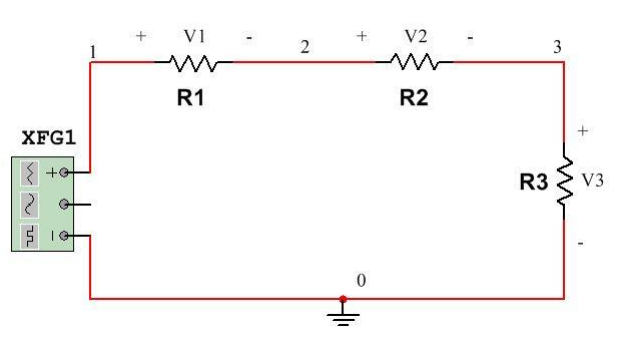
\includegraphics[width=0.75\textwidth]{img/c1.png}
  \end{figure}

  \item Make the following connections between the Analog Discovery pins and the nodes on the
  board:
  \begin{itemize}
    \item 1 – WaveGen1, W1 (Solid Yellow Line)
    \item 1 – Scope Channel, 1+ (Solid Orange)
    \item 0 – Ground (Black)
    \item 0 – Scope Channel, 1- (Striped Orange)
  \end{itemize}

  \item Activate the Digilent Waveforms button which would display a window (Digilent
  WaveForms 1) as shown in Figure~\ref{fig:dadwg}. The first step is to adjust the WaveGen.
  Click on the WaveGen button and set the arbitrary waveform generator to generate a DC
  voltage of amplitude 0 volts and 0 offset.
    \begin{figure}[!ht]
  \centering
  \caption{Digilent Analog Discovery WaveGen setup\label{fig:dadwg}}
  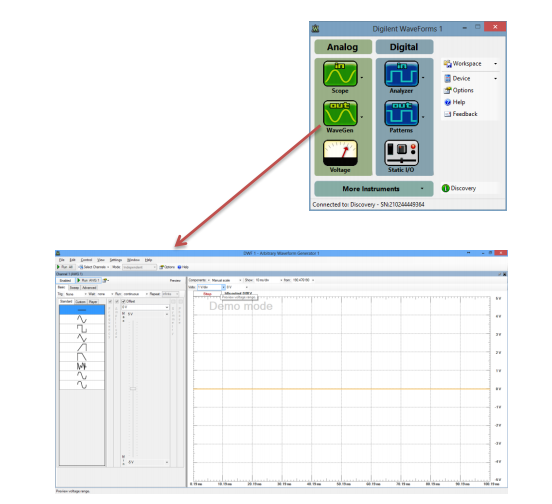
\includegraphics[width=0.75\textwidth]{img/awg.png}
  \end{figure}



  \item After making the adjustments on wave generator click the Run AWG1
  \item To observe the output, activate the voltmeter by clicking on the Voltmeter under the
  More Instruments tab.
  \item Record the voltage across the resistor and fill in the table as the voltage source varies from
  0 to 5 V. Replace resistor R1 with R2 and fill in Table 3 by varying the voltage source from 0 to 5
  V.
\end{enumerate}
\vspace{1cm}

\subsection{Part B: Investigation of Electric Power Transfer}
\label{sub:Procedure Part B}
\begin{enumerate}
  \item Build the circuit shown in Figure~\ref{fig:maxpowerschem}  on the bread board.
    \begin{figure}[!ht]
  \centering
  \caption{Schematic for Measuring Maximum Power Transfer\label{fig:maxpowerschem}}
  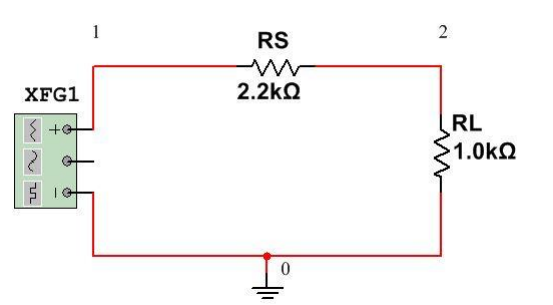
\includegraphics[width=0.75\textwidth]{img/c2.png}
  \end{figure}

  \item Make the following connections between the Analog Discovery pins and the nodes on the
  board:
  \begin{itemize}
    \item 1 – WaveGen1, W1 (Solid Yellow Line)
    \item 2 – Scope Channel, 1+ (Solid Orange)
    \item 0 – Scope Channel, 1- (Striped Orange)
    \item 0 – Ground (Black)
  \end{itemize}
  \item Activate the Digilent Waveforms button which would display a window (Digilent
  WaveForms 1) as shown in Figure~\ref{fig:dadwg}. The first step is to adjust the WaveGen.
  Click on the WaveGen button and set the arbitrary waveform generator to generate a DC
  voltage of amplitude 5 volts and 0 offset.
  \item After making the adjustments on wave generator click the Run AWG1
  \item To observe the output, activate the voltmeter by clicking on the Voltmeter under the
  More Instruments tab.
  \item Record the voltage across the load resistor ($R_L$) and the current through the load resistor
  ($R_L$).
  \item Replace the first load resistor with the second load resistor and record the values in the
  table. Repeat this process till all the resistances are filled.
  \item Make the necessary calculations (Equation \ref{eq:1}) to complete the rest of the table and plot efficiency ($\eta$) as a
function of the load resistance.
  \begin{equation}
    \begin{gathered}
      P_L = V_L \times I_L \\
      P_{in} = V_S \times I_L \\
      \eta = 100 \times \frac{P_L}{P_{in}}
    \end{gathered}\label{eq:1}
  \end{equation}



\end{enumerate}
  \clearpage

  \section{Results}
  \label{sec:results}
  

\subsection{Setup}
\label{sub:Setup}
Resistors were provided, a total of 11. They were then documented by
their bands and values in Table~\ref{tab:resultResistors}.
    \begin{table}[!ht]
  \captionsetup{font=large}
  \centering
  \caption{ List of Resistors Used }
  \label{tab:resultResistors}
  \begin{tabular}{   | l | c | c | c | r | }
  \hline

      Resistor &     Color Code &     Calculated Value ($ k \Omega $) &     Measured Value ($ k \Omega $)     \\ \hline
      1 &    Brown Black Red Gold &     1 &     0.99     \\ \hline
      2 &    Red Red Red Gold &     2.2 &     2.18     \\ \hline
      3 &    Brown Black Brown Gold &     0.1 &     0.099     \\ \hline
      4 &    Blue Blue Red Gold &     6.8 &    6.8     \\ \hline
      5 &    Brown Black Black Gold &     0.01 &     0.01     \\ \hline
      6 &    Orange Orange Red &     3.3 &    3.25     \\ \hline
      7 &    Brown Green Red Gold &     1.5 &    1.46     \\ \hline
      8 &    Yellow Purple Black Gold &     0.047 &     0.046     \\ \hline
      9 &    Orange White Black Gold &     0.039 &     0.039     \\ \hline
      10 &    Red Purple Black Gold &     0.027 &     0.027     \\ \hline
      11 &    Red Black Black Brown Brown &     2 &     2      \\ \hline
  
  \end{tabular}
  \end{table}




\subsection{Part A: Verification of Ohm’s law}
\label{sub:Part A}
      
      \begin{table}[!ht]
  \captionsetup{font=large}
  \centering
  \caption{ Verification of Ohm's Law using resistor $R_1$ }
  \label{tab:ohm1}
  \begin{tabular}{   | l | c | c | r | }
  \hline

      Source Voltage ($V_s$) &     $V_{R1}$ (V) &    $I_{R1}$ (mA)     \\ \hline
      0 &    0.0 &    0     \\ \hline
      0.5 &     0.492 &    0.492     \\ \hline
      1 &    0.992 &    0.992     \\ \hline
      1.5 &    1.492 &    1.492     \\ \hline
      2 &    1.992 &    1.992     \\ \hline
      2.5 &    2.493 &    2.493     \\ \hline
      3 &    2.995 &    2.995     \\ \hline
      3.5 &    3.491 &    3.491     \\ \hline
      4 &    3.990 &    3.99     \\ \hline
      5 &    4.990 &    4.99     \\ \hline
  
  \end{tabular}
  \end{table}



      
      \begin{table}[!ht]
  \captionsetup{font=large}
  \centering
  \caption{ Verification of Ohm's Law using resistor $R_2$ }
  \label{tab:ohm2}
  \begin{tabular}{   | l | c | c | r | }
  \hline

      Source Voltage ($V_s$) &     $V_{R2}$ (V) &    $I_{R2}$ (mA)     \\ \hline
      0 &    0.0 &    0     \\ \hline
      0.5 &     0.492 &    0.224     \\ \hline
      1 &    0.992 &    0.451     \\ \hline
      1.5 &    1.493 &    0.679     \\ \hline
      2 &    1.993 &    0.906     \\ \hline
      2.5 &    2.494 &    1.134     \\ \hline
      3 &    2.995 &    1.361     \\ \hline
      3.5 &    3.493 &    1.588     \\ \hline
      4 &    3.991 &    1.814     \\ \hline
      5 &    4.990 &    2.268     \\ \hline
  
  \end{tabular}
  \end{table}



\begin{enumerate}
  \item The unknown resistors are made of linear material which can be seen from their graphs in Figures~\ref{fig:plot1} and \ref{fig:plot2} .
  The graph indicates linearity by the fact that the trend line matches the
  samples points without diverging or deviating.
    \begin{figure}[!ht]
  \centering
  \caption{Plot of Verification of Ohm's Law using resistor $R_1$\label{fig:plot1}}
  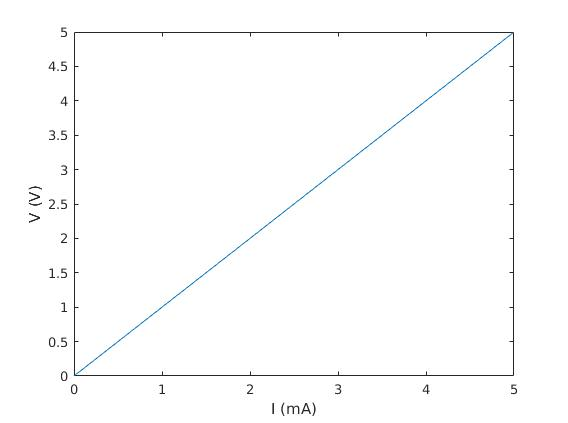
\includegraphics[width=0.65\textwidth]{img/plot1.jpg}
  \end{figure}

    \begin{figure}[!ht]
  \centering
  \caption{Plot of Verification of Ohm's Law using resistor $R_2$\label{fig:plot2}}
  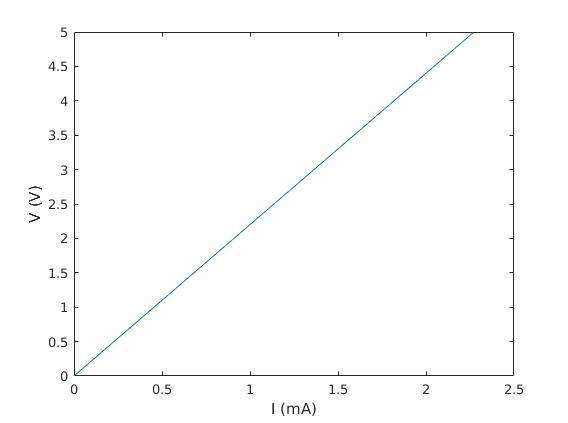
\includegraphics[width=0.65\textwidth]{img/plot2.jpg}
  \end{figure}

  \item $R_1$ and $R_2$ can be calculated by the slope of the IV graph.
  From the slope the resistances were calculated to be 1k, and 2.2k which is the
  the same as their resistance rating. Despite high accuracy there is low precision as
  the linear regression was done with a simple best fit line.
  \begin{gather}
    m = \frac{y_2-y_1}{x_2-x_1} = \frac{1.0 V - 0.0 V}{1.0 mA - 0.0 mA} = 1000 \frac{V}{A} = 1 k \Omega \\
    m = \frac{y_2-y_1}{x_2-x_1} = \frac{1.1 V - 0.0 V}{0.5 mA - 0.0 mA} = 2200 \frac{V}{A} = 2.2 k \Omega
  \end{gather}
\end{enumerate}

\vspace{1cm}

\subsection{Part B: Investigation of Electric Power Transfer }
\label{sub:Part B}
      
  
  
      \begin{table}[!ht]
  \captionsetup{font=large}
  \centering
  \caption{ Determination of maximum power transfer }
  \label{tab:maxpower}
  \begin{tabular}{   | l | c | c | c | c | c | r | }
  \hline

      $R_L(k \Omega)$ &     $V_L(V)$ &     $I_L(mA)$ &    $P_L$ (mW) &    $P_{in}$ (mW) &    Efficiency (\%)     \\ \hline
      6.8 &    3.78 &    0.5 &    1.89 &    2.5 &    75.6     \\ \hline
      3.3 &    2.99 &    0.86 &    2.571 &    4.3 &    59.8     \\ \hline
      2 &    2.38 &    1.14 &    2.713 &    5.7 &    47.6     \\ \hline
      1.5 &     2.00 &    1.32 &    2.64 &    6.6 &    40     \\ \hline
      1 &     1.568 &    1.51 &    2.368 &    7.55 &    31.36     \\ \hline
      0.1 &     0.217 &     2.13 &    0.462 &    10.65 &    4.34     \\ \hline
      0.047 &     0.103 &     2.19 &    0.226 &    10.95 &    2.06     \\ \hline
  
  \end{tabular}
  \end{table}



\begin{enumerate}
  \item \begin{itemize}
    \item As the load resistance increases the load voltage increases.
    There is a direct non-linear relationship between voltage and resistance. This can be seen by the blue line of plot
    figure \ref{fig:currentvoltage}.
    \item As the load resistance increases the load current decreases.
   There is a indirect non-linear relationship between current and resistance. This can be seen by the red line of the plot.
   \end{itemize}
  The graph indicates:
  \begin{equation}
    \text{ As } R_L \to \infty \hspace{1cm} \begin{matrix}
    V_L \to V_{in} = 5 V \\
    I_L \to 0
  \end{matrix}
  \end{equation}
  Testing various resistor values in the voltage divider equation yeilds the same
  values that were measured.
  \begin{gather}
    \text{For a voltage divider: } V_{out} = V_{in} \cdot \frac{R_L}{R_S+R_L} \\
    V_{out}(R_L \to 0) = (5 V) \cdot \frac{0}{(2.2 k \Omega)+0} = 0 \\
    V_{out}(R_L \to 6.8k ) = (5 V) \cdot \frac{6.8 k \Omega}{(2.2 k \Omega)+ 6.8 k \Omega} = 3.78V
  \end{gather}



    \begin{figure}[!ht]
  \centering
  \caption{Plot of Voltage and Current as a Function of Load Resistance $R_L$\label{fig:currentvoltage}}
  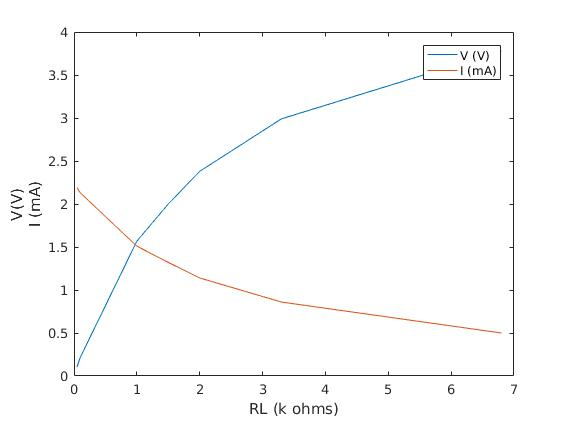
\includegraphics[width=0.75\textwidth]{img/plotc.jpg}
  \end{figure}


  \item The load power increased as the load resistance increased till it reached a maximum.
  At this point the power decreased. It created a concave down curve represented in Figure~\ref{fig:loadpower}
    \begin{figure}[!ht]
  \centering
  \caption{Plot of Load Power $P_L$ as a Function of Load Resistance $R_L$\label{fig:loadpower}}
  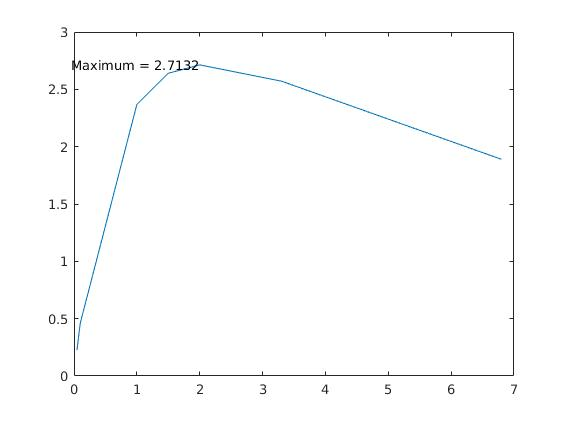
\includegraphics[width=0.7\textwidth]{img/plotd.jpg}
  \end{figure}


  \item The resistor that resulted in the maximum power transfer was the $2.0 k\Omega$
    resistor, but according to the regression of the plot (Figure~\ref{fig:loadpower}) the value would be $R_L = 2.7 k\Omega$
    Both these values fall close to the value of the source resistor which
    had a value of $R_s = 2.2 k\Omega$. To be consistent with the theorem for maximum
    power transfer the load resistor would be equal to the source resistance $R_S$.
  \item The resistor that resulted in the maximum efficiency was the $6.8k \Omega$
  resistor, but according to the regression of the plot (Figure~\ref{fig:loadeff}) the value would
  be $R_L = 75.6 k\Omega$. However, these points were the endpoints of the sample data
   and the plot respectively. In reality the maximum efficiency is only when the resistance
   reaches infinity. The end behavior of the graph indicates this by the horizontal asymptote at $100\%$.
   \[\text{As } R_L \to \infty , \eta \to 100\% \]
     \begin{figure}[!ht]
  \centering
  \caption{Plot of Efficiency $\eta$ as a Function of Load Resistance $R_L$\label{fig:loadeff}}
  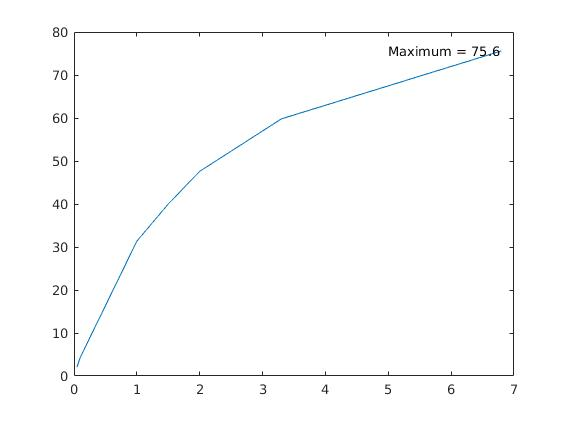
\includegraphics[width=0.7\textwidth]{img/plote.jpg}
  \end{figure}


\end{enumerate}
  \clearpage

  \section{Discussion}
\label{sec:Discussion}
After completing the experiments it was found that the resistors
provided did indeed obey ohm's law. A simple plot proves this because
the current and voltage was linear which. This was expected because there
is no reason why ohm's law wouldn't apply to simple resistors. Originally
the instructions were misunderstood. The error was that the current through the
resistor did not need to be measured. Furthermore, the Digilent Analog
Discovery board could not measure current. Instead, the current was measured
using the ELVIS II board.

For the power transfer circuit it was found that the voltage across
the load resistor had a direct relationship to the resistance, and the current an indirect
relationship. The calculations showed that maximum power transfer happens when the
load resistance is equal to that of the source resistance, and when the efficiency is at 50\%.
The maximum efficiency would be when the circuit is left unconnected where the resistance is
at its largest. This was expected as well, because prior knowledge lead to the
hypothesis that the maximum is the same is that thevenin resistance. The prelab
exercise also involved simulating the same experimental which lead to the same
results.

\section{Conclusion and Recommendations}
\label{sec:Conclusion}
This experiment was a valuable introduction to Digilent Analog Discovery board
and served its purpose to become familiar with the platform. The lab reveal any
new knowledge about circuitry as the experiments yielded the same results as
hypothesized. In the future the lab could have been done better if done using
equipment that can measure current. This was a minor setback that required
introducing new equipment to take up this task. This lab was helpful and will
provide a sound step in the following labs that build off of these experiments.
  \clearpage

  \begin{thebibliography}{9}
    \bibitem{manual}
    Dr. Petru Andrei, Ifedayo Ogundana, and Jose Cordova.
    \textit{Lab 1 DC Circuits I: Voltage, Current, Resistance, Ohm’s Law, and Electric Power}
  \end{thebibliography}



\end{document}
